\documentclass[12pt]{article}
\usepackage[utf8]{inputenc}
\usepackage[english]{babel}
\usepackage{graphicx}
\usepackage{dirtytalk}
\usepackage[export]{adjustbox}
\usepackage{wrapfig,blindtext}
\setlength{\parindent}{0em}
\setlength{\parskip}{1em}

\title{COVID-19 Open Data : Map-Reduction and Visualisation}
\author{Tafara Freddie Hove \\
        \small u18278150 \\
}
\date{}

% K
\providecommand{\keywords}[1]
{
  \small	
  \textbf{\textit{Keywords---}} #1 
}

\begin{document}
\maketitle
\begin{abstract}


Big data  causes many challenges to conventional data analysis and mining  techniques due to its characteristics like volume, velocity and variety. Hence, there is need for more advanced technologies that can process and analyse Big data  effectively and efficiently. This report discusses the COVID-19 Data, which Big Data and how  to use Apache Spark on such datasets. Applying analytical techniques to big data can help extract valuable information that can be used to monitor and manage the spread of COVID-19  pandemic. Data analysis and visualisation will be done on the selected attributes using Apache Spark.

\end{abstract}\hspace{10pt}
\keywords{COVID-19, Apache Spark, Map-reduce, Visualisation}

\section{INTRODUCTION}

Apache Spark is a distributed computing  technology that processes large datasets. A Mapreducing model works on Apache Spark to analyze data. Mapreduce is very efficient for batch processing and it can be implemented on Apache Spark which is very efficient for iterative in-memory computing. It supports distributed and parallel applications that handle large quantities of data. Mapreduce is a software framework  that can process massive datasets in a distributed environment over several devices \cite{}. Hence it is  required to analyze COVID-19 data to give insight about the patterns and trends of active, confirmed, recovered and deceased cases in the world and South Africa in particular.

 Mapreduce involves the mapping the data in a collection of (key, value) pairs and reducing all the pairs using the same key. Map function can do grouping, filtering and sorting of data. On the other hand, reduce function aggregates and summarizes the data results generated by the map function. In the project we analyze and visualize the COViD-19 Open dataset, an open data source  which can help about a better understanding of health status of the world at large. Processing and analysing Big Data on a local machine using traditional techniques such as excel posses a big challenge since the local machines dont have the capacity to process the data.
 
 In order to  have a perspective of the world health issues related to COVID-19 there are question that are going to be dicussed and answered during the data analysis and visualisation.
 
 This paper is giving a comprehensive examination of of the CIVID-19 Open dataset using Apache Spark processing tools. It discuses the processes, approaches,results and visuals of the executed operations. The paper's layout is as follows ; Section 2 --------

\section{DATASET}
 In this  section, a detailed overview of the COVID-19 open dataset is presented. The dataset reveals main aspects of COVID-19. The section explains the dataset, highlighting some key interesting characterstics and discuss some attributes that possess some interesting aspects  within the dataset.

\subsection{Dataset overview}

 As discussed in PART 1 of the this project;  COVID-19 Open Data is a huge dataset that consists of country-level datasets of daily time-series data about COVID-19 worldwide \cite{covid-19}.The repository contains datasets of more than 50 countries around the world for the timespan February 2020 to date. The data is disaggregated  by country or by regions. The datasets reveal the impact of the virus and how different countries are responding to the pandemic.  It contains the latest available public data on COVID-19 including a daily situation update, the epidemiological curve and the global geographical distribution \cite{covid-19}. The COVID-19 Open Data is available at https://github.com/GoogleCloudPlatform/covid-19-open-data. This is dataset is made up of live data files in the Google Cloud directory.

The COVID-19 Open Data is collected from multiple sources such as Wikidata, DataCommons, WorldBank, University of Oxford and Google. The data is sourced from different countries through the initiative of the World Health Organisation's Epidemic Intelligence on daily basis. The data reports are based on the number of COVID-19  confirmed, recovered, tested and deaths cases, from health authorities worldwide to mention but a few. Hence the dataset is a resource of multiple types of data outcomes, static co-variate data, dynamic co-variate data and dynamic intervention state data\cite{covid-19}.The data is stored in separate CSV and JSON files which are published in Google Cloud Storage. The collection of such huge quantities of files constitutes 1.01GB of data.  The merged datasets' size has  more than 6112480 observations and 45 attributes.  The attributes types are strings and numeric values. The dataset that is stored on BiQuery Puplic dataset program.

\subsection{Features Selection}
Feature selection is a process where a subset of attributes or variables of a dataset are selected for further processing to address the task at hand. The attributes which are  not having interesting information are removed. New  attributes can also be created and added to the data frame. Hence the  attributes  of interest were selected from the dataset for data analysis using Apache Spark.  Such data analysis using the selected attributes was used to calculate and determine needed measures to curb the spread of the pandemic and its devastating consequences. They also reveal the relationship between the spread of the virus in a country and how people's lives and livelihoods are being affected.

Below is a list of selected variables and reason their inclusion in the data analysis:

\begin{itemize}
    \item date: This is the day a COVID-19 case was recorded or confirmed. It helps to monitor the trends (increases/decrease in number of cases) of the pandemic. For each date, the cumulative number of confirmed cases and deaths as reported that day in that county or state are shown. All cases and deaths are counted on the date they are first announced.
    
    \item country name: The column reveals names of countries and which countries are making progress against the pandemic. It shows what measures implemented by a country in response to the pandemic.
    
    \item region1 name:  The column illustrates states/provinces of different countries and how each geographic area responds to the pandemic.
    
    \item cumulative confirmed: This column shows the total number of recorded positive cases from the day the first case was recorded. 
      
    \item cumulative deceased:  Is the total deaths from coronavirus recorded. Help to check if the number of deaths are increasing or decreasing, compared to other countries. This shows if the country is able to contain the pandemic or not? Is the death toll continues to rise quickly daily or weekly?
    
    \item cumulative recovered: The number of total number of people infected and recovered from coronavirus.
      
     \item cumulative test:  It shows how much testing for coronavirus do countries conduct, when it started how does it compared with other countries? if the number of confirmed cases is lower than the actual cases , then it means that there is limited testing in that country.
      
    \item new confirmed cases: These are the recently new cases of the virus that emerged in a location/country. It reveals how the country performs test relative to the size of the outbreak.
    
\end{itemize}


\subsection{Investigative Questions}

\begin{enumerate}
    \item Which  countries have the highest number of commutative confirmed, cumulative deceased and recovered cases?
    \item  Which countries have the highest active cases ?
    \item How does the number of confirmed cases correspond to hospitalizations and deaths?
    \item how does economic actives, people mobility and recreation where affected by the pandemic?
    \item Which provinces in South Africa has the  confirmed cases highest cases ?
    \item Is the spread of COVID-19 associated with weather condition (temperature)?
    \item has the number of infections changed over time in  USA countries?
\end{enumerate}

In order to address the questions  defined above  some  data manipulation, processing and analysis was data on the defined Apache Spark environment as discussed in the next section.

\section{METHODOLOGY}
Apache Spark open source platform was used for processing data on the Google Cloud Platform. Spark is fast, scalable, fault tolerant and distributed. Mapreduce framework efficiently distributes the job over a number of commodity hardware and calculate the result in parallel. However some procedures wereimplemented before data analysis as revealed below:

\subsection{ Google Cloud Dataproc Cluster Setup}
Firstly, the project was created on Google Cloud platform console. The cloud storage bucket to be used on the Dataproc cluster was created to store data files from BigQuery . The Python 3 kernel was used to configure the SparkSession on the Jupyter notebook.  Thus the gloogle cloud platform was used for Spark needs.

The Dataproc hadoop cluster with Apache Spark was setup on the three nodes with one master (namenode) and two worker nodes(datanodes). The cluster was created in a defined region and zone. Each node had 2V CPU3.75GB n1-standard core, and 32GB disk size storage capacity. Then the latest version of hadoop 2.9 and spark 2.4 was used to setup the cluster. In a dataproc hadoop cluster, the jupyter notebook for python was was also accessed for the processing of big data.  In the dataproc cluster notebook the spark-bigquery-connector and BigQuery Storage API were used to  load data into the Spark Cluster. Then the Spark data from can be created by reading in data from the public BigQuery dataset. 

\subsection{ Exploratory Data Analysis}
Data exploration analysis is the very first and critical step in data analysis process. It involves the exploring of the data to identity the data patterns, trends, variable characteristics and other interesting points. it helps to understand the key concepts and issues of the data so as to get a better informed representation of the entire dataset. Through data exploration on notebooks the dimensions of the dataset and the variable types were identified. Hence the data set was cut into a manageable size, focusing on analyzing the most relevant attribute discussed in section II. 

\subsection{Data preparation}
 This is a data extraction process which involves data preparation activities such cleaning, transforming and rearranging of data. The dataset had missing data and duplicate data. The duplicate rows were removed, and missing values were replaced. Some features were selected and some were drop for data analysis. Hence the data was rearranged in various ways to ensure  manipulation of datasets. 


\subsection{Spark SQL}
Spark is an efficient and fast engine used to process and analyze large-scale data. It is an in-memory computation hence it was chosen over Hadoop Map-Reduce which read  and write to a disk which makes slow. Spark SQl and Spark RDDs are the key technologies for data analysis in Spark. The data analysis in Spark ais  executed through pipelining using transformation and action operations. To ensure effective COVID-19 data analytics using Spark Mapreduce the number of operations were implemented. Moreover, in this project Spark SQL was used for querying  and analyzing the dataset. SQL can easily  query DataFrames and familiar queries can also be executed on top of park for data analysis.

\section{ANALYSIS AND RESULTS}

This section presents the results of analyzed attributes extracted from the dataset. The purpose is to reveal the project findings  in relation to the insights that were mined from the data. As discussed in the last section, Spark SQL was used to query the dataset to answer the  investigative questions highlighted in the previous section. The graphs and maps will clearly illustrate the findings and solutions to the  questions in the next section.  

\begin{enumerate}
    \item cumulative confirmed, cumulative deaths  and cumulative recoveries
    The result of the project shows that  from top 20 countries with high cumulative conformed cases, they have also very high deaths. For instance United States of America has a total of 9126351 confirmed cases and 230556, followed by india with 8184082 confirmed cases and 122111 deaths. In Africa, the most affected country is South Africa with 725452 cumulative confirmed cases and 19276 death cases. Seemingly this reveals that as more people get infected with COVID-19 virus a sizeable numbered of people is expected to die. In addition the findings also showed that more people were hospitalized.On the other hand the number of confirmed cases depend on the number of test done in the country.The countries have very high number of people who tested for COVID-19.  Hence there is a high correlation between cumulative confirmed and  cumulative deceased cases. 
    
    \item Active cases
    The active case finding is another key for the control and prevention communicable diseases. By removing deaths and recoveries from confrimed cases gives the actual currently infected cases or what is called active cases. The active cases are fluctuating day by day and country by country.  But  there statistics revealed that country with high active cases have also high deaths and hospitalisations like USA, UK, Spain and South Africa.
    
    The prediction of active cases is a very crucial measure used to evaluate the current COVID-19 situation. Every active case can lead to the infection of more people hence contributing to danger in the future. When the active cases decrease it implies a less danger in the  exponential spread of COVID-19
    
    \item Cases in South Africa
    South Africa is the country in Africa with the highest number of  COVID-19 infections. South Africa COVID-19 data was extracted from the main dataset. The statistics revealed that more cases were concentrated in Gauteng with 228756 confirmed cases and Western Cape recorded 117 326.  The percentage ratio of the cases are as follows ----. In addtion high  number of hospitalisations and death cases are also confirmed in these provinces. 
    
    
    \item Checking trends on the number of new infections per pay in SA in the past 100 days
    The aim is to analyze the patterns in the last 100 days  to check whether the infections are increasing or decresing in South Africa.
     
     \item Temperature vs Confirmed cases
     The aim was to corelate tempretaute and transmission. 
    
\end{enumerate}

\section{VISUALISATION}
Visualisation is a significant aspect of big data analysis process. Informative visualisation identifies patterns and establishes trends of big data. Big data is messy, it is difficult to analyze and understand. There there is need for data visualization techniques for effective communication of data. The main objective of using data visualisation in this project is to simplify quantitative information of COVID-19 Open data through visuals such as graphs and maps. The relationships, characteristics and patterns underlying data will be revealed through maps and plotting. Hence the  hidden patterns. The novel big data visualisation techniques extract hidden patterns, trends and ensure clear cut understanding of the dataset. The data quries built in SQL language were used to retrieve insightful information from the data
\
Since this section is a follow-up of the prevision section on data analysis and results some of the processed outcomes will be visualized in this sections. The packages that were used for data visualization include searbon, matplotlib, and pandas to mention but a few. The forms of analysis presentation are visual graphs, charts and maps.

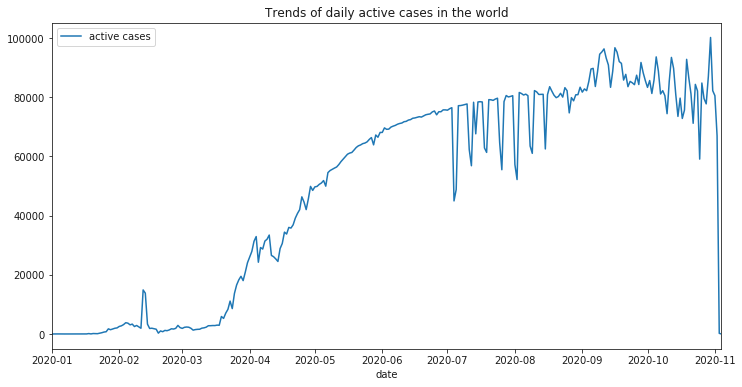
\includegraphics[width=0.9\textwidth,inner]{activecases.png}
\caption{Fig 1: Line graph showing the trends of active cases in the world.}

What we observed  from Figure 1 is that the active cases is increasing over time since the begging of the pandemic. For entire of January to March the active number of active cases was constant except a for a sharp increase and decrease in mid February. A continuous rapid increase in the cases started in mid March  until end of June. The exponential increase continue but with some deep drops in between until October.  The drops could be a result of lockdown inposted by many countries and other regulations such as the use of face masks and sensations. The  rapid  fluctuation  active cases could be also be due to relaxation of regulations by many countries and people ignorance to abide by COVID-19 regulations. The rapid vertical decline of the line graph at the end of time period is a result of incomplete data. The data of the present day is not yet updated hence the graph drops to zero. 


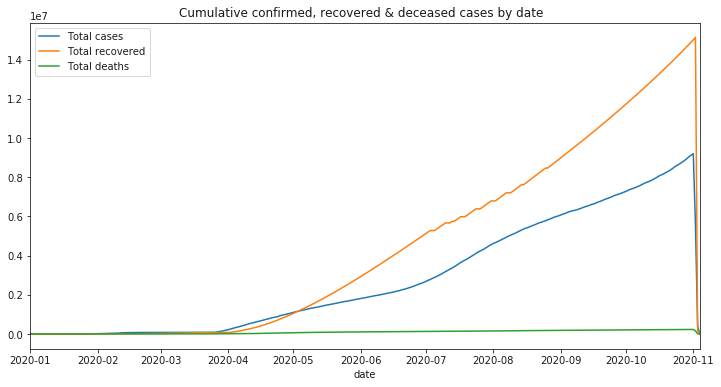
\includegraphics[width=0.9\textwidth, inner]{line2.png}
\caption{Fig 2: Line illustrating the relationship among the cumulative confirmed deceased and recovered.}

Figure 2 depicts the cumulative frequencies of confirmed, deceased and recovered cases for the whole world as from January to date.  The graphs show that
The graph shows that about 75 million cases of coronavirus cases were reported as of October 30, 2020, with more than 100m recoveries and about 700000 thousand fatalities. Between April and mid May the number of confirmed  cases was higher than the number recovered. But subsequently, the recovery rate increased rapidly, exceeding the total confirmed cases. This shows that most countries took precaution measured to ensure high recovery rate. The rate of deaths was showed a very limited gradual increase until the end of the period. However it is difficult to give a conclusion of who did mot since the age groups re not published in this data set.  

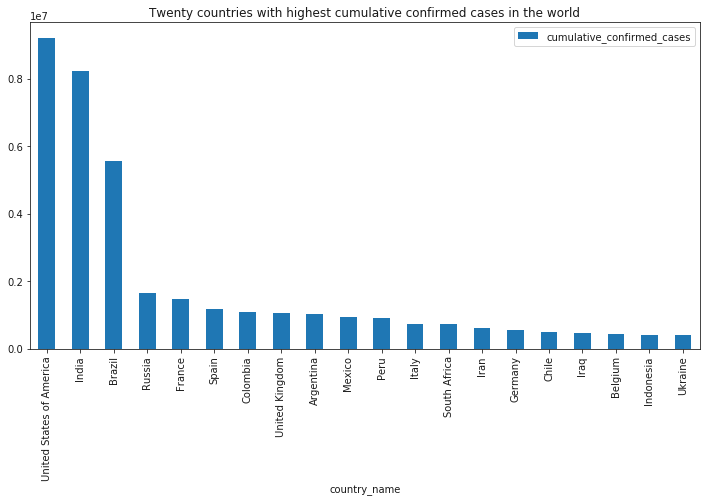
\includegraphics[width=0.9\textwidth, inner]{bar1.png}
\caption{Bar graph showing countries with highest number of cumulative confirmed cases}


Figure 3 shows that United States of America is the most affected country in the world with more than 9million people contracted the virus. In addition, India and Brazil also recorded very high infections, 8.3million and 5.8million respectively. In Africa, South Africa is the most affected country with more than 730000 thousand confirmed cases. The countries with high confirmed cases have also very high number of tests conducted, compared most country with very low figures and minimal tests conducted. 


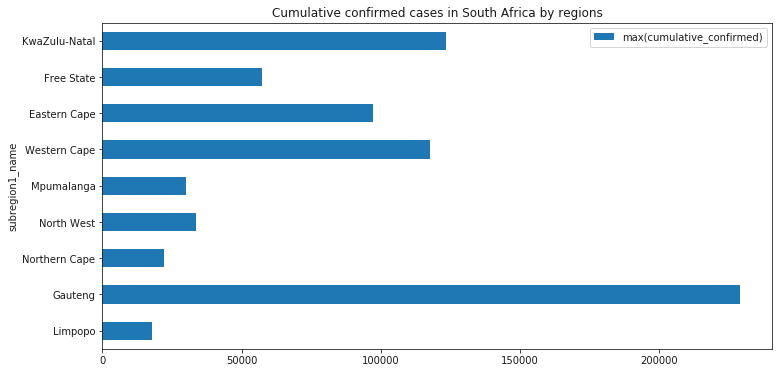
\includegraphics[width=0.9\linewidth, inner]{bar2.png}
\caption{Fig 4: Bar graph showing cumulative confirmed cases in provinces of South Africa }

south Africa has nine provinces, Figure 4 above shows the total confirmed cases of each province. Gauteng and Western Cape have have been witnessing very high surges since the beginning of the pandemic. They recorded 230000 and 117000 respectively. On the other hand Mpumalanga, Northern Cape and Limpopo have least number of cases recorded. This shows that the hardest hit province are those with large cities. This is where most cases  of COVID-19 emerge. The factors contributing to this could be inward migration and increased congregations in high density areas causing cluster outbreaks since social distancing is impossible to practise. 


\centering
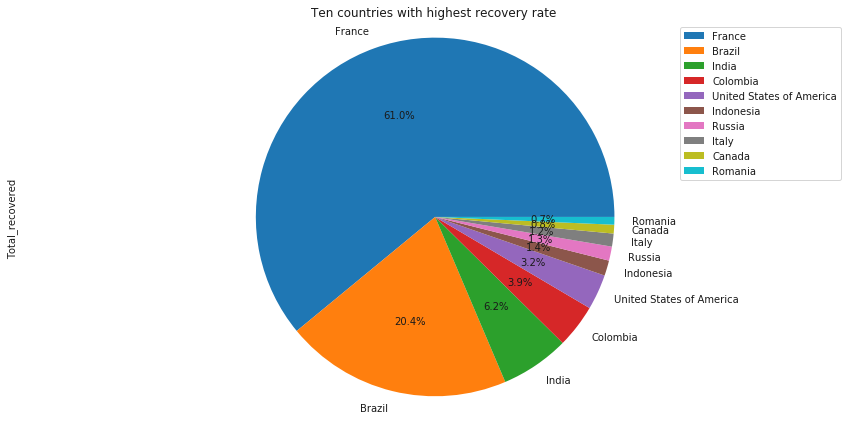
\includegraphics[width=0.9\textwidth, inner]{pie1.png}
\caption{Fig 5: Pie chart showing the distribution of cumulative recoveries on ten countries}


Figure 5 shows the percentage of recoveries of the cumulative cases in the world. From the ten selected countries France has the highest proportion of 61 percent, followed by Brazil with 20 percent and India has 6 percent. This means that in theses countries even though many people are being infected they are recovering from the from the effects of the virus.

\centering
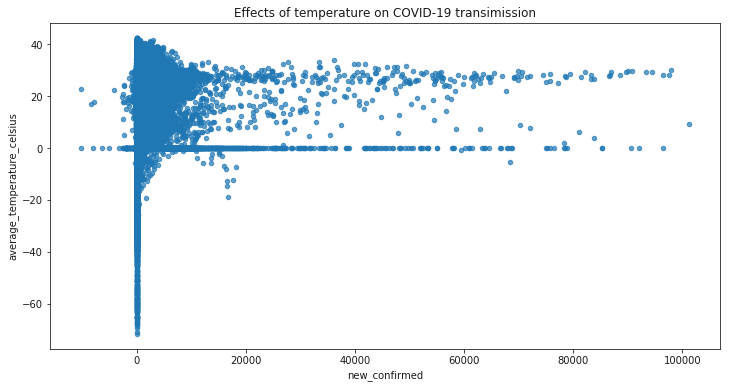
\includegraphics[width=0.9\textwidth, inner]{scatter.png}
\caption{Fig 6: Scatter plot showing the effect of temperature on virus transmission.}

The effect of temperature on Virus on the transmission of the virus is shown in Figure 6 above.
We investigate whether cumulative  cases of coronavirus in the world to check whether the rate of transmission of the virus declines at higher temperature. The graphs are not showing either a negative correlation or positive correction between the two variables. There were assumptions that the rate of transmission is very high in winter and very low in summer. There is no evidence  that a higher average temperature reduces the incidence of cases of the virus the country. WE can conclude that with this trends there is no co relation between seasonal increases in temperature and coronavirus 

\centering
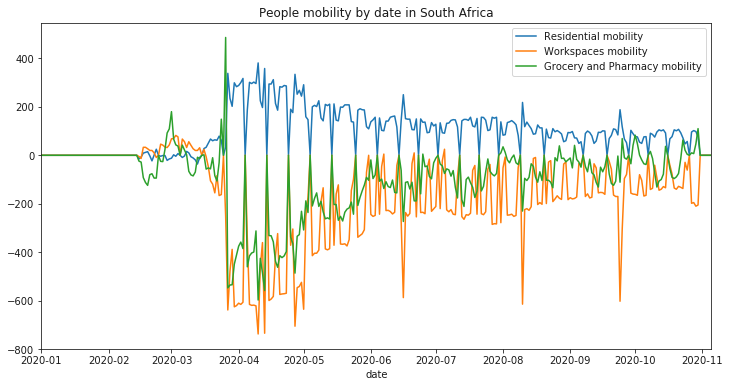
\includegraphics[width=0.9\textwidth, inner]{mobility.png}
\caption{Fig 7: Scatter plot showing the effect of temperature on virus transmission.}

Figure 7 illustrates how the community in South Africa is moving around differently since the beginning of the spread of the virus. The line graphs are providing insights into what has changed in communities in the country in response to regulations implement by the government to combat COVID-19. 

\end{document}















